\section{Heurística de Búsqueda Tabú}
\subsection{Implementación del Algoritmo}

\par{La implementación de la heurística de búsqueda tabú es muy similar a la
implementación de la heurística de búsqueda local. La vecindad se definió
de la misma forma (con $V$ como parámetro). Al pseudocódigo de búsqueda local
se le agregó todo lo referente a la lista tabú, además de la definición de un
criterio de terminación. A continuación se muestra el pseudocódigo de la
heurística.}\\

\begin{algorithm}[H]
	\caption{Pseudocódigo de la heurística de búsqueda tabú}
	\KwData{\textbf{Grafo} $G(V,E)$, \textbf{Solucion} $solucion\_inicial$}
	\textbf{Solucion} $solucion\_optima$ $\leftarrow$ $solucion\_inicial$\\
	\textbf{Solucion} $solucion\_actual$ $\leftarrow$ $solucion\_inicial$\\
	\While{No se alcance el criterio de terminación}{
		\textbf{Solucion} $mejor$\\
		\For{( \textbf{Solucion} $temporal$ $\in$ Vecindad($solucion\_actual$) )}{
			$solucion\_optima$ $\leftarrow$ Max($solucion\_optima$, $temporal$)\\
			\If{$\neg$EsTabu($temporal$)}{
				$mejor$ $\leftarrow$ Max($mejor$, $temporal$)
			}
		}
		EsTabu($solucion\_actual$)\\
		$solucion\_actual$ $\leftarrow$ $mejor$\\
	}
	\textbf{return} $solucion\_optima$
\end{algorithm}

\par{La variable $solucion\_optima$ guarda la mejor solución encontrada hasta
el momento. La variable $solucion\_actual$ guarda la solución sobre la que se
está iterando. Mientras no se alcance el criterio de terminación, se recorre
toda la vecindad de la $solucion\_actual$. Para cada solución vecina, se
evalúa si es mejor que la $solucion\_optima$ hallada hasta el momento. Si lo
es, la reemplaza. Luego se evalúa si es un candidato a ser la próxima
$solucion\_actual$. Para ello debe ser mejor que la $mejor$ vecina de la
$solucion\_actual$. Si lo es y no es una solución tabú, pasa a ser la nueva
$mejor$. Una vez obtenida la $mejor$ solución vecina de $solucion\_actual$,
se agrega a $solucion\_actual$ a la lista tabú, para no volver a caer en ella
y se le asigna a $solucion\_actual$ el valor de la solución vecina $mejor$.}\\

\par{Para determinar la mejor entre dos soluciones se utiliza la función $Max$,
la cual obtiene el tamaño de la frontera de las soluciones que compara. A las
soluciones inválidas (que no representan cliques en el grafo) se les asigna
un valor negativo, para que sólo puedan ser elegidas como $mejor$ si no hay
ninguna otra válida que pueda ser tomada. No se corren riesgos de devolver una
solución inválida, ya que la $solucion\_optima$ se inicializa con la
$solucion\_inicial$ que se asume válida (y por lo tanto con frontera mayor o
igual a cero) y $solucion\_optima$ solo se actualiza con soluciones mejores
estrictamente. Sí es posible que $solucion\_actual$ tome un valor inválido,
pero esto ayuda a diversificarse cuando se está estancado.}\\

\par{Aunque no figura en el pseudocódigo, la implementación también puede
llegar a tomar una solución tabú como $solucion\_actual$ si no puede tomar
ninguna otra. Si bien se estaría regresando a una solución ya evaluada,
en esta segunda iteración sobre esa solución se espera que se diversifique
en lugar de quedarse ciclando entre un conjunto acotado de soluciones, ya
que el resto de las soluciones ya recorridas también pertenecen a la lista
tabú y solo deberían volver a recorrerse si no hay opciones que no sean
tabú.}\\

\par{La lista tabú se implementó como una clase (en el archivo $tabu\_list.h$)
que almacena una cantidad determinada de soluciones. Implementa las funciones
$add\_tabu$ para agregar una solución a la lista y $es\_tabu$ que determina si
una solución pertenece a la lista. Se la inicializa con el tamaño máximo, es
decir con la cantidad de soluciones que puede almacenar. Ese valor es
parámetro de la implementación. Cuando la lista se
llena, reemplaza la nueva solución con la solución más vieja de la lista.
Sin embargo, cuando se llama a $es\_tabu$ se altera el orden de la lista para
poner como más nueva la solución que se evalúa. De esta forma, se conservan
soluciones viejas que podría ser necesario evaluar próximamanete ya que
pertenecen a la vecindad de la $solucion\_actual$.}\\

\par{El criterio de terminación se basa en un contador que determina cuántas
iteraciones se realizaron sin que mejore la $solucion\_optima$. Cuando la
solución óptima se actualiza por una solución mejor, el contador se reinicia.
Cuando el contador llega a un máximo, el cual es pasado como parámetro, el
ciclo de iteraciones termina y se devuelve la $solucion\_optima$ almacenada.
Esta implementación debe terminar ya que $solucion\_optima$ sólo se actualiza
con soluciones estrictamente mejores y el tamaño de la frontera máxima es
acotado, por lo tanto, no puede seguir creciendo indefinidamente y no pueden
pasar infinitas iteraciones con la misma $solucion\_optima$.}

\subsection{Orden de complejidad}

\par{La complejidad del algoritmo depende de tres elementos. Estos son la
máxima cantidad de iteraciones sin mejora permitidas ($I$), el tamaño de la
lista tabú ($T$) y el tamaño de la vecindad ($V$). A continuación se analizará
cada uno por separado:}
\\\\
\textbf{Máxima cantidad de iteraciones sin mejora $I$}\\

\par{Es evidente que el valor de $I$ es determinante a la hora de calcular la
complejidad. El ciclo principal (líneas 3 a 10 del pseudocódigo) itera sobre
el valor de la variable $iter$\footnote{ver código: función $tabu$ en el
archivo $tabu.h$} la cual se inicializa en $0$ y se incrementa en cada
iteración. El ciclo itera mientras la variable $iter$ sea menor a $I$. Sin
embargo, hay que tener en cuenta también que la variable $iter$ se reinicia
cada vez que se encuentra una solución mejor (estrictamente) a la óptima.
Esto sólo sucede con soluciones estrictamente mejores, por lo que la cantidad
de veces que la variable $iter$ se reinicia está acotada por el valor de la
frontera máxima del grafo, el cual a su vez, está acotado por la cantidad de
aristas. En el peor caso, cada vez que $iter$ está por alcanzar el valor de
$I$, se reinicia, por lo tanto la máxima cantidad de iteraciones del ciclo
principal es $m*I$ con $m$ la cantidad de aristas.}\\

\par{Esta cota es muy poco ajustada, ya que sólo podría darse
con un grafo que tenga una clique cuya frontera sea todas las aristas del
grafo. En dicho caso, la clique solución no podría contener aristas y por lo
tanto sería un solo nodo adyacente a todos los demás, en otras palabras, una
estrella. Pero si fuese ese el caso, entonces no es posible reiniciar el valor
de $iter$ m veces, ya que no existen cliques con fronteras de tamaños
intermedios entre 1 y m-1, exepto claro estrellas de menos de 4 aristas.
También hay que tener en cuenta que se parte de una solución inicial (aunque
su valor de frontera podría ser cero), por lo que una cota más ajustada
es $(m-f_i)*I$ con $f_i$ el tamaño de frontera de la solución inicial, la cual
sigue siendo del orden de $m*I$.}
\\\\
\textbf{Tamaño de la lista Tabú $T$}\\

\par{El valor de $T$ influye tanto positiva como negativamente a la complejidad.
Cada vez que se evalúa si una solución pertenece a la lista tabú esta debe, en
el peor caso recorrerse toda. Por lo que la función $esTabu$ tiene una
complejidad de $T$ y debe evaluarse para cada solución en cada vecindad cada
iteración. Esto ya le da a la implementación una complejidad de $\#i*\#v*T$ con
$\#i$ la cantidad de iteraciones del ciclo principal y $\#v$ la cantidad de
vecinos de la vecindad. Se ve que la complejidad es directamente proporcional
al valor de $T$, sin embargo un valor pequeño de $T$ también podría incrementar
la cantidad de iteraciones $\#i$ del ciclo principal. Si se está recorriendo
una vecindad con muchas soluciones con el mismo tamaño de frontera es posible
que la $mejor$ solucion sea una tabú. Si la lista tabú es suficientemente
grande, podrá almacenar a todas estas soluciones y rápidamente diversificarse
a otra vecindad lejana. Si la lista tabú no permite almacenar todas estas
soluciones, empezarán a sobreescribirse, lo que produciría que la
implementación se quede recorriendo varias veces el mismo conjunto de
soluciones y tarde más en diversificarse (o peor, que consuma todas las
iteraciones en ese conjunto acotado de soluciones y termine su ejecución
antes de diversificarse).}\\

\par{Se ha implementado si embargo una pequeña mejora para reducir la
posibilidad de $estancamiento$. Esto es que, al llamar a la función $esTabu$
para la solución $S$, si se encuentra esa solución, se reubica al frente de
la lista. Si bien no aporta una mejora considerable, ayuda a que no se quiten
de la lista elementos que es probable que se vuelvan a necesitar (si $S$
pertenece a la vecindad de la $solucion\_actual$ es probable que pertenezca
también a la vecindad de la siguiente solución que se tome como
$solucion\_actual$).}
\\\\
\textbf{Tamaño de la vecindad $V$}\\

\par{El ciclo principal itera $\#i$ veces. Luego recorre los $\#v$ elementos de
la vecindad de la\\$solucion\_actual$. La función $obtener\_vecino$ es la misma
que la utilizada en la heurística de búsqueda local\footnote{implementada en el
archivo $grafo.h$}, por lo que la complejidad es la misma y vale el mismo
análisis realizado en la sección de complejidad de búsqueda local. Recordamos
que se considerará la complejidad en función de $V$ con $F(V)$,
si bien es cierto que, formalmente, esta complejidad está acotada superiormente
por $2^n$.}\\
 
\par{Finalmente, la complejidad de la implementación de búsqueda tabú es\\
$(m-f_i)*I * F(V) * V*\Delta(G) * T \in$ O($m*I*2^n*n*T$). Si bien esta
complejidad parece excesiva para una heurística (de hecho es mayor a la
complejidad de evaluar todas las soluciones), hay dos razones que nos llevan a
pensar que en la práctica se comportará mejor. En primer lugar, deben tomarse
instancias muy específicas (o parámetros muy malos) para que la cantidad de
iteraciones se acerque a $m*I$. Es esperable que, de haber muchas soluciones
vecinas mejores la implementación converga más rápido a soluciones óptimas y
no que itere sobre $I$ soluciones iguales o peores antes de mejorar. Incluso
es probable que al tomar una solución vecina, se consiga una de frontera varias
veces mayor y no necesariamente mejorar siempre de a uno.}\\

\par{En segundo lugar, la elección de los parámetros $I$, $T$ y $V$.
Con un tamaño de vecindad de $V = 1$, la cantidad de vecinos de cada solución es
$F(1) = \binom{n}{1} = n$ la cual es una buena cantidad de vecinos y
resulta en una complejidad de O($m*I*n*n*T$). A su vez, el tamaño de la lista
tabú no tiene porqué ser demasiado grande. Con $T = n^2$ se obtiene una
lista considerablemente grande. La cantidad de aristas $m$ se puede acotar por
$n^2$ y el valor de $I$ podría ser una constante como $100$ o $1000$. Con estos
valores, la complejidad sería $n^2 * 1000 * n * n * n^2 \in$ O($n^6$), es decir,
es polinomial. Incluso si $V$ fuese 2 o 3 los tiempos de ejecución tampoco se
acercarían a la complejidad del algoritmo exacto.}

\subsection{Comportamiento}

\par{La complejidad de la búsqueda tabú no se ve tan influenciada por la
elección de la solución inicial como en el caso de la búsqueda local. La
heurística de búsqueda tabú permite tomar como solución actual soluciones
peores o incluso inválidas, por lo que es menos probable que se estanque como
la búsqueda local. Aún así, la cota inferior a la frontera de la solución
devuelta también es la frontera de la solución inicial, ya que en el peor caso,
esta no encuentre ninguna mejor. Sí depende de los parámetros $I$, $T$ y $V$, los
cuales determinan cuántas iteraciones se realizarán y cuántas soluciones se
evaluarán en total.}

\subsection{Experimentación}

\subsubsection{Performance}

\par{El archivo $test\_tabu.cpp$ en la carpeta $codigo/tabu$ contiene la
implementación del código que mide los tiempos de ejecución de la heurística
de búsqueda tabú. Se ejecutó este programa con $N$ = 1200, $s$ = 20 y $k$ = 10.
Es decir, para cada $n$ entero múltiplo de 20, entre 20 y 1200, se generaron
10 grafos aleatorios (con la función $generar\_aristas\_aleatorias$). Para cada
instancia generada se corrieron tres versiones de la heurística de búsqueda
tabú. Con V=1, con V=2 y con V=3. Para las tres, la solución inicial fue la
solución vacía, tanto el tamaño de la lista tabú como la cantidad máxima de
iteraciones sin mejorar fueron $n$.
En el siguiente gráfico se muestran los resultados obtenidos.}

\begin{center}
\textbf{Gráfico de performance de la heurística de búsqueda tabú\\ en
función de la cantidad de nodos del grafo}
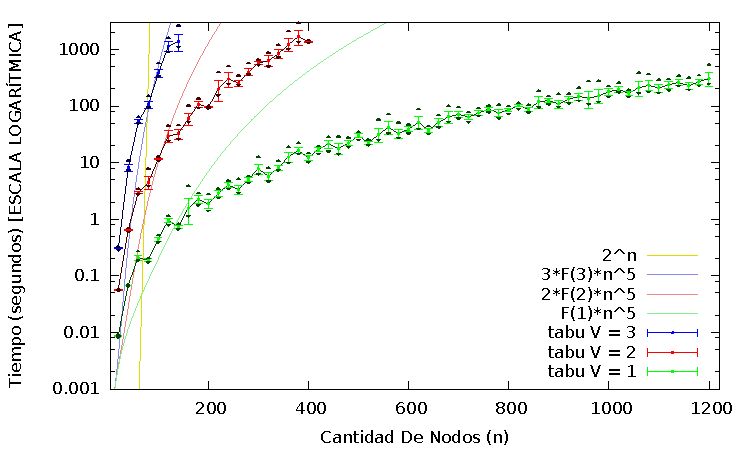
\includegraphics[scale=1.3]{imgs/tabu_1200_20_10.pdf}
\end{center}

\par{Cada punto $\bullet$ en el gráfico representa el promedio de los tiempos
medidos para cada una de las 10 ejecuciones de una determinada cantidad de nodos
del grafo. El tamaño del segmento vertical sobre cada punto $\bullet$ representa
su varianza asociada. Además, para cada cantidad de nodos $n$ se graficaron la
máxima medición con $\blacktriangle$ y la mínima medición con
$\blacktriangledown$.}\\

\par{La función graficada con una curva amarilla es una función exponencial de
base 2. Al estar utilizando escala logarítmica en el eje de ordenadas, esta curva
se ve como una recta. También se graficaron otras tres funciones para que acoten
superiormente cada una de las heurísticas, basándose en su complejidad estimada
en función de $F(V)$. Como se puede observar, si bien incrementando el $V$ los
tiempos de ejecución de la heurística aumentan considerablemente, están muy
lejos de asemejarse a la curva de la función exponencial\footnote{Para que
las comparaciones tengan sentido, las cuatro funciones graficadas fueron
multiplicadas por las mismas constantes. Es por ello que fue difícil ajustar
las tres cotas superiores a las curvas definidas por las tres heurísticas.},
la cual se ve en el gráfico como una recta casi vertical.}

\subsubsection{Optimalidad}

\par{El archivo $opt\_tabu.cpp$ en la carpeta $codigo/tabu$ contiene la
implementación del código que mide el índice de optimalidad de la heurística
de búsqueda tabú. Se ejecutó este programa con\\$N$ = 100\footnote{Para el test
de performance ejecutamos instancias de tamaño 1200. Sin embargo, para calcular
la optimalidad de la heurísica también debemos ejecutar el algoritmo exacto
con cada instancia, lo que nos restringe el máximo tamaño de entrada.},
$s$ = 2 y $k$ = 10. Es decir, para cada $n$ entero par entre 2 y 100, se
generaron 10 grafos aleatorios (con la función $generar\_aristas\_aleatorias$).
Para evaluar como afecta al índice de optimalidad cada uno de los parámetros
($V$ y $T$) por separado, se corrieron para cada parámetro, tres variantes
sobre ese parámetro manteniendo constante el otro. A continuación se
evalúa cada uno por separado. En los test de performance sólo se evaluó la
influencia de $V$ porque ya estaba claro como el valor de $T$
influía sobre la complejidad, no es así sobre el índice de optimalidad.}
\\\\
\textbf{Tamaño de la vecindad $V$}\\

\par{Para cada instancia generada se corrieron las mismas tres variantes que
en el test de performance. Con V=1, con V=2 y con V=3. Para las tres, la
solución inicial fue la solución vacía, tanto el tamaño de la lista tabú
como la cantidad máxima de iteraciones sin mejorar se mantuvieron constantes en
$n$. Para que los datos no se amontonen, utlizamos $s$ = 2 en lugar de $s$ = 1.
En el siguiente gráfico se muestran los resultados obtenidos.}

\begin{center}
\textbf{Gráfico de optimalidad de la heurística de búsqueda tabú
en función\\de la cantidad de nodos del grafo (variando el tamaño de la
vecindad $V$)}
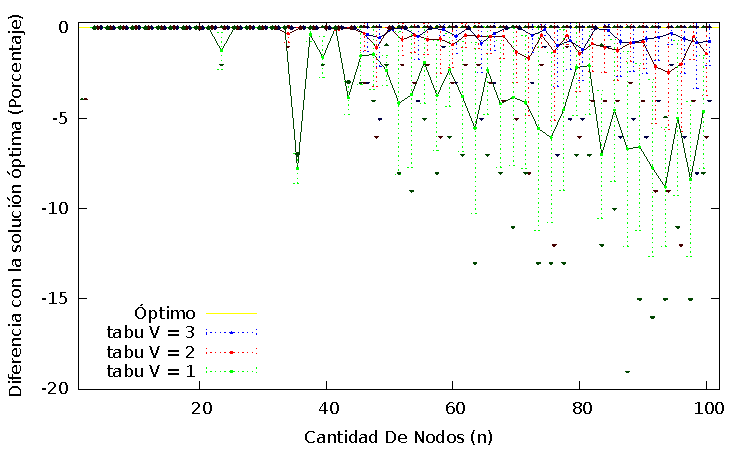
\includegraphics[scale=1.3]{imgs/opt_tabu_100_2_10.pdf}
\end{center}

\par{Cada punto $\bullet$ en el gráfico representa el promedio del índice de
optimalidad para cada una de las 10 ejecuciones de una determinada cantidad de
nodos del grafo. El tamaño del segmento vertical (en líneas punteadas, también
para que los datos no se amontonen) sobre cada punto $\bullet$
representa su varianza asociada. Además, para cada cantidad de nodos $n$ se
graficaron la máxima medición con $\blacktriangle$ y la mínima medición con
$\blacktriangledown$.}\\

\par{La recta $y=0$ representa la solución óptima, así que cuanto más se
asemeje la curva definida por una heurística a dicha recta, mejor es la
heurística. Como se puede observar, para pequeños valores de $n$ las tres
variantes de la heurística encuentran siempre, o casi siempre, una solución
óptima. Al aumentar la cantidad de nodos, aumentan tanto la diferencia
respecto a la solución óptima, como la varianza asociada.}\\

\par{En el caso de la heurística de búsqueda local, la variante con $V$=3 era
claramente superior a las otras dos en cuanto a optimalidad, y las otras dos
eran bastante similares. En el caso de la heurística de búsqueda local es la
variente con $V$=1 la que es claramente distinta (esta vez por ser inferior)
mientras que las variantes con $V$=2 y $V$=3 son bastante similares. En
promedio, la variante con $V$=3 es ligeramente superior, aunque en determinados
casos es inferior a la variante con $V$=2, por lo que no se ve una mejora
considerable por parte de la variante con $V$=3 respecto a la variante
con $V$=2.}\\

\par{Incluso para $n$ mayores, hay instancias para las que las tres variantes de
la heurística encuentran una solución óptima, de hecho para la mayoría de los $n$
hay al menos una instancia para cada variante tal que la variante encuentra
una solución óptima. Esto se ve en los $\blacktriangle$ de las tres variantes
que están sobre la curva $y=0$. Aunque para los mismos $n$ hay instancias en
que la solución devuelta por la variante con $V$=1 difiere en más del 15\% del
óptimo. No es así con las variantes con $V$=2 y $V$=3, cuyos mínimos
en dichos casos difieren en pocos casos en más del 10\% respecto a la solución
óptima. Como esperábamos, la varianza en el índice de optimalidad de la heurística
es muy grande debido a que este depende mucho del tipo de grafo que resuelve.
Al incrementar la cantidad de nodos, las curvas definidas por los resultados de
los algoritmos parecen estabilizarse. En promedio las variantes con $V$=2 y
$V$=3 parecen encontrar soluciones que representan entre el 1\% y el 5\% del
óptimo, mientras que la variante con $V$=1 parece estabilizarse entre el 5\% y
el 10\%. También parece que ninguna de las tres variantes es peor del 20\%.}
\\\\
\textbf{Tamaño de la lista Tabú $T$}\\

\par{Para cada instancia generada se corrieron tres variantes de la heurística.
Con T=$\sqrt{n}$, con T=$n$ y con T=$n^2$. Para las tres, la
solución inicial fue la solución vacía, la cantidad máxima de iteraciones sin
mejorar se mantuvo constante en $n$, mientras que el tamaño de la vecindad se
mantuvo constante en $1$. Para que los datos no se amontonen, utlizamos $s$ = 2
en lugar de $s$ = 1.
En el siguiente gráfico se muestran los resultados obtenidos.}
\newpage
\begin{center}
\textbf{Gráfico de optimalidad de la heurística de búsqueda tabú
en función\\de la cantidad de nodos del grafo (variando el tamaño de la
lista tabú $T$)}
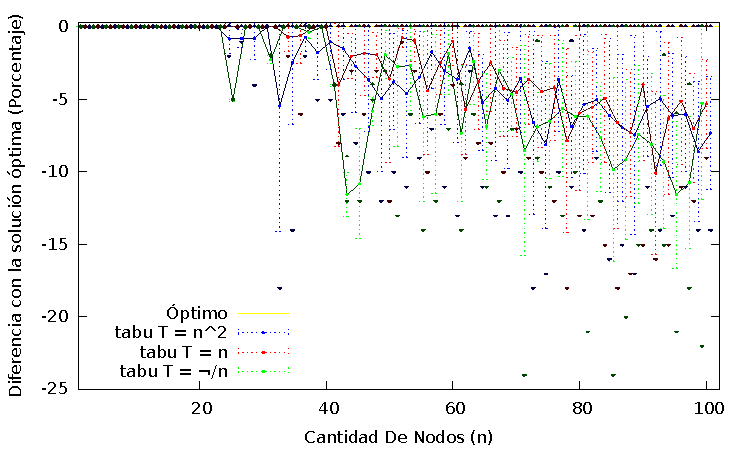
\includegraphics[scale=1.3]{imgs/opt_tabu_T_100_2_10.pdf}
\end{center}

\par{Cada punto $\bullet$ en el gráfico representa el promedio del índice de
optimalidad para cada una de las 10 ejecuciones de una determinada cantidad de
nodos del grafo. El tamaño del segmento vertical (en líneas punteadas, también
para que los datos no se amontonen) sobre cada punto $\bullet$
representa su varianza asociada. Además, para cada cantidad de nodos $n$ se
graficaron la máxima medición con $\blacktriangle$ y la mínima medición con
$\blacktriangledown$.}\\

\par{La recta $y=0$ representa la solución óptima, así que cuanto más se
asemeje la curva definida por una heurística a dicha recta, mejor es la
heurística. Como se puede observar, para pequeños valores de $n$ las tres
variantes de la heurística encuentran siempre, o casi siempre, una solución
óptima. Al aumentar la cantidad de nodos, aumentan tanto la diferencia
respecto a la solución óptima, como la varianza asociada.}\\

\par{En cuanto al parámetro $V$, era claro que incrementarlo producía
mejores resultados. En el caso del parámetro $T$, ninguna de las tres
variantes es claramente superior. Las curvas definidas por ellas se
entrecruzan constantemente, por lo que no es claro cual de las tres
es mejor. Al parecer depende mucho del tipo de grafo entrada y no de
la cantidad de nodos del mismo.}\\

\par{Incluso para $n$ mayores, hay instancias para las que las tres variantes de
la heurística encuentran una solución óptima, de hecho para la mayoría de los $n$
hay al menos una instancia para cada variante tal que la variante encuentra
una solución óptima. Esto se ve en los $\blacktriangle$ de las tres variantes
que están sobre la curva $y=0$. Aunque para los mismos $n$ hay instancias en
que las soluciones difieren en más del 15\% del óptimo. Como esperábamos, la
varianza en el índice de optimalidad de la heurística es muy grande debido a que
este depende mucho del tipo de grafo que resuelve. En este caso no queda claro
que las curvas definidas por los resultados tiendan a estabilizarse al rededor
de un determinado porcentaje de diferencia con el óptimo, pero al menos parece
que ninguna de las tres variantes es peor del 25\%.}
